\chapter{Моделирование процессов хемотаксиса бактерий}\label{ch:ch2}

\section{Моделирование процесса генерации степенных распределений на основе механизма дискретного белкового шума}\label{sec:ch2/sec1}
Внутриклеточные сигнальные пути формируют сеть для управления движением бактерии с использованием информации о градиенте концентрации веществ во внеклеточном пространстве. Сеть сигнальных путей процесса хемотаксиса у бактерий E.~coli состоит из небольшого числа компонент, однако этого оказывается достаточно для проявления некоторых свойств сложных биосистем, таких как адаптация и ответ на внешний стимул \cite{korobkova_molecular_2004}. В своей работе авторы показали, что шум, создаваемый сигнальными сетевыми взаимодействиями, контролирует поведенческую вариабельность. Этот механизм демонстрирует свойство биологической системы адаптироваться за счет контроля молекулярного шума. 

Сигнальная сеть хемотаксиса начинается с процесса связывания молекул хемоаттрактанта с сайтами хеморецепторов на цитоплазматической мембране бактерии. Далее, каскад внутриклеточной сигнализации управляет производством белка CheY-P, который диффундирует к моторам и модулирует переключение направления вращения. Изменение направления вращения жгутиков по часовой стрелке (CW) на вращение против часовой стрелки (CCW) заставляет бактерии менять свой паттерн движения: с вращения на одном месте к прямолинейному движению.

Значительный прогресс в понимании статистики переключения двигателей был достигнут с помощью минимальной модели, учитывающей переходы между двумя состояниями через энергетический барьер \cite{tu_how_2005}. Регулирующий путь сводился к действию фосфорилированной формы сигнальной молекулы CheY-P, так что более высокая концентрация CheY-P приводила к более высокой вероятности перехода CCW в CW \cite{khan_steady-state_1980}. В этой работе было обнаружено, что гауссовский шум с конечным временем корреляции может приводить к масштабированию распределений длительностей вращения моторов против часовой стрелки. Подобные флуктуации может вызывать внутренняя стохастичность сигнального генетического пути, в частности, <<генетический шум>> связанный с конечным числом реагирующих белковых молекул.

Для демонстрации возможности возникновения переключений с промежуточной степенной статистикой в связи с генетическим шумом в данном разделе рассматривается модель химической кинетики синтеза белка CheY-P и возникающего в результате переключения вращения моторов. 

Рассмотрим минимальную модель сигнального пути с точки зрения химической кинетики. Переходы между различными значениями числа молекул белка CheY-P, обозначенного $Y$, задаются следующим уравнением:
\begin{equation}
    \begin{aligned}
        Y \mathrel{\mathop{\rightleftarrows}^{\mathrm{K_{y}^{+}}}_{\mathrm{K_{y}^{-}}}} Y + 1
    \label{eq:chem}
    \end{aligned}
\end{equation}

где $K_{y}^{+}=\frac{Y_0}{\tau}$, $K_{y}^{-}=\frac{Y+1}{\tau}$ -- коэффициенты интенсивностей перехода между состояниями, $Y_0$ -- равновесное число молекул, $\tau$ -- характерное время релаксации сигнального пути к равновесному числу молекул. Являясь элементарным процессом рождения-смерти, по своей сути содержит все необходимые свойства: стохастичность, дискретность состояний и конечное время корреляции $\tau$. Значение $Y_0$ можно принять постоянным в связи с тем, что концентрация хемоаттрактанта изменяется медленно (в процессе движения клетки в слабом градиенте или при изменении уровня хемоаттрактанта во времени) по сравнению со шкалой времени переключения. 

По аналогии рассмотрим модель переключения вращения жгутиков. Пусть $X = 0$ соответствует режиму вращения по часовой стрелке, а $X = 1$ — против часовой стрелки:
\begin{equation}
    \begin{aligned}
        X \mathrel{\mathop{\rightleftarrows}^{\mathrm{K_{x}^{+}}}_{\mathrm{K_{x}^{-}}}} X + 1
    \label{eq:turning}
    \end{aligned}
\end{equation}
где коэффициенты $K_x^{+}=K^{+}(1-X)$, $K_x^{-}=K^{-}X$ ограничивают состояния $X={0, 1}$ и переходы контролируются состоянием регулирующего белка CheY-P через соответствующие интенсивности переключения:
\begin{equation}
    \begin{aligned}
        K^{\pm}=K_0 \exp(\pm\alpha^\pm \cdot \frac{Y_0-Y}{Y_0})
    \label{eq:turning-rates}
    \end{aligned}
\end{equation}
где $\alpha^\pm>0$ характеризует чувствительности интенсивностей переходов, при этом энергетические барьеры аппроксимируются линейной зависимостью относительно уровня CheY-P \cite{khan_steady-state_1980}.

Опишем качественное поведение предложенной модели. Пусть жгутики вращаются по часовой стрелке, что соответствует вращению бактерии на одном месте: $X=0$, а интенсивности соответственно равны $K_x^{+}=K^{+}$ и $K_x^{-}=0$. При уровне белка CheY-P ниже равновесного состояния $Y<Y_0$ интенсивность (частоту) переключения в сторону вращения жгутиков против часовой стрелки (то есть прямолинейного движения бактерии) доминирует: $K^{+}>K_0$. Большие значения уровня белка CheY-P $Y>Y_0$, наоборот уменьшает интенсивность (частоту) переключений. Соответственно при вращении жгутиков против часовой стрелки смещение уровня белка выше или ниже равновесного состояния приводит к обратному эффекту. Отличающиеся друг от друга уровни интенсивности в свою очередь позволяют независимо настраивать интенсивности переходов между движение бактерии вперед и вращением на месте.

Однако в рассмотренной модели есть недостаток: интенсивности переходов могут принимать значения экспоненциально большие или экспоненциально малые в ответ на изменение концентрации $Y$, что может быть биологически неправдоподобным. В соответствии с работой \cite{frankel_adaptability_2014} для учета конечного числа связываний белков CheY-P с моторами, интенсивности переходов могут быть заменены на:
\begin{equation}
    \begin{aligned}
        K^{\pm}=K_0^{\pm} \exp \left (\pm\frac{\alpha^\pm}{2} \left (\frac{1}{2} - \frac{Y}{Y+K_d} \right ) \right )
    \label{eq:turning-rates-kd}
    \end{aligned}
\end{equation}
Такие коэффициенты соответствуют насыщению с уровнем числа белков, превышающем константу диссоциации $K_d$.

Исследование статистических свойств модели было выполнено с помощью численного моделирования уравнений \cref{eq:chem,eq:turning,eq:turning-rates,eq:turning-rates-kd} с применением стохастического алгоритма Гиллеспи \cite{gillespie_stochastic_2007}. В результате численных расчетов был получен набор реализаций, состоящих из $N=10^7$ шагов, соответствующих одной из возможных химических реакций. Один из типов реакции это переключение направления вращения моторов (уравнение \cref{eq:turning}). Непрерывные участки времени пребывания в каждом состоянии CW и CCW соответственно (между переключениями моторов) обозначим $\{t_{ccw}\}$ и $\{t_{cw}\}$. Всего было собрано не менее $N_{cw} = N_{ccw} = 10^{10}$ отрезков времени пребывания в состояниях CW и CCW.

Полученные выборки были использованы для оценки функций плотности вероятности $p(t_{cw})$ и $p(t_{ccw})$ и проанализированы зависимости от времени релаксации сигнального пути $\tau$ и чувствительности интенсивностей переходов между состояниями $\alpha^{\pm}$. Полученные функции плотности вероятности были аппроксимированы степенной функцией на отрезке $[a, b]$ с использованием линейной регрессии в двойном логарифмическом масштабе методом наименьших квадратов. Качество аппроксимации оценивалось коэффициентом детерминации \cite{magnus_2021}, $R^2 \in [0, 1]$. Отрезок $[a, b]$ выбирался перебором с условиями: длина отрезка не менее $1.3$ декады и коэффициент детерминации $R^2 > 0.98$. Если такой отрезок не был найден, то гипотеза об участке со степенным распределением отвергается. 

Рассмотрим простую форму интенсивностей, заданной уравнением \cref{eq:turning-rates}, и оценим плотности вероятности длительностей для соответственно двух состояний CW (вращение бактерии на одном месте) и CCW (прямолинейное движение). В случае отсутствия молекул CheY-P, $Y=0$ (переключение нечувствительно к CheY-P, $\alpha_{\pm}=0$), процесс является пуассоновским, а плотности вероятности длительностей пребывания в состояниях экспоненциальны, $p(t_{ccw}), p(t_{cw}) \propto \exp(-K_0 t)$.

Далее проводился численный анализ для случая равных чувствительностей переключения $\alpha_\pm = \alpha$. Численные результаты показывают, что коррелированный молекулярный шум дает степенное распределение длительностей, $p(t_{ccw}) \approx t^{-\gamma}$, в четко выраженном интервале (1.5-2 декады) с отсечкой при больших значениях. продолжительность (Рис. \cref{fig:duration-pdf}а).
Плотности с промежуточной степенной асимптотикой на более чем 2 декадах и затухающей с почти экспоненциальной отсечкой, типичны как для измерений in vivo и in vitro пространственной активности бактерий \cite{korobkova_molecular_2004,harris_generalized_2012}.

\begin{figure}[ht]
    \begin{minipage}[b][][b]{0.49\linewidth}\centering
        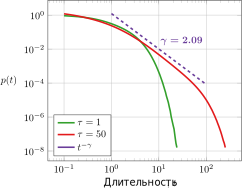
\includegraphics[width=1\linewidth]{genetic-noise/ru/fig1a} \\ а)
    \end{minipage}
    \hfill
    \begin{minipage}[b][][b]{0.49\linewidth}\centering
        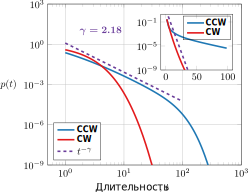
\includegraphics[width=1\linewidth]{genetic-noise/ru/fig1b} \\ б)
    \end{minipage}
    \caption{
        (а) Плотности вероятности длительностей в состоянии CCW для различных значений времени релаксации белка CheY-P, $\tau$. Остальные параметры: $\alpha = 10$, $Y_0 = 20$, $K_0 = 1$; (б) Плотности вероятности длительностей CW и CCW для $\alpha^+ = 1$, $\alpha^- = 10$, $Y_0 = 20$, $\tau = 50$, $K_0 = 1$. Штриховыми линиями обозначены участки со степенной асимптотикой с показателями $\gamma = 2.09$ (а) и $2.18$ (б), коэффициент детерминации которого $R^2 = 0.98$, количество реализаций $N_{ccw} = N_{cw} = 10^{10}$, $t \in [1, 100]$. На вставке повторно представлены плотности вероятностей длительностей с логарифмической шкалой по оси ординат.
    }
    \label{fig:duration-pdf}
\end{figure}


В работе \cite{tu_how_2005} аналогично было показано, что уменьшение времени корреляции изменяет это распределение в сторону экспоненциального. Рассмотренная модель также способна воспроизводить экспоненциальную статистику длительности CW одновременно со степенным распределением длительностей CCW. При этом, распределения различны из-за несовпадающих чувствительностей интенсивностей переходов между состояниями, то есть $\alpha_+ \neq \alpha_-$. Поскольку время пребывания в состоянии определяется интенсивностью (частотой) покидания этого состояния, то снижение чувствительности перехода из CW в CCW к уровню белка CheY-P должно приводить к экспоненциальному распределению длительностей CW подобно предельному случаю $\alpha^+ = 0$. На рисунке \cref{fig:duration-pdf}б продемонстрирован пример данного режима системы.

Численное моделирование в широком диапазоне параметров показывает, что степенные распределения возникают только тогда, когда время релаксации уровня CheY-P существенно больше, чем время переключения между состояниями CW и CCW $\tau \gg \frac{1}{K_0}$ (Рис. \cref{fig:pdf-gamma-grid-1}а,б). В то же время, увеличение среднего числа сигнальных молекул $Y_0$, приводит к отклонению гипотезы о степенном распределении (Рис. \cref{fig:pdf-gamma-grid-1}а,б). Увеличение числа сигнальных молекул приводит к относительному уменьшению флуктуаций, что в свою очередь уменьшает влияние генетического шума. Параметр чувствительности $\alpha$ контролирует переход между степенным и экспоненциальным распределением длительностей (Рис. \cref{fig:pdf-gamma-grid-1}а). Значения показателя степени $\gamma$, найденные в большей части области параметров ($1 < \gamma < 3$) согласуются с экспериментальными наблюдениями, которые оценили степенной показатель для кумулятивного распределения длительностей CCW как $\gamma - 1 \approx 1.5$. Это свидетельствуют о том, что медленное метилирование как часть сигнального пути отвечает за длительные временные корреляции в выходном сигнале, что приводит к степенному распределению длительностей \cite{korobkova_molecular_2004}. 


\begin{figure}[ht]
    \begin{minipage}[b][][b]{0.49\linewidth}\centering
        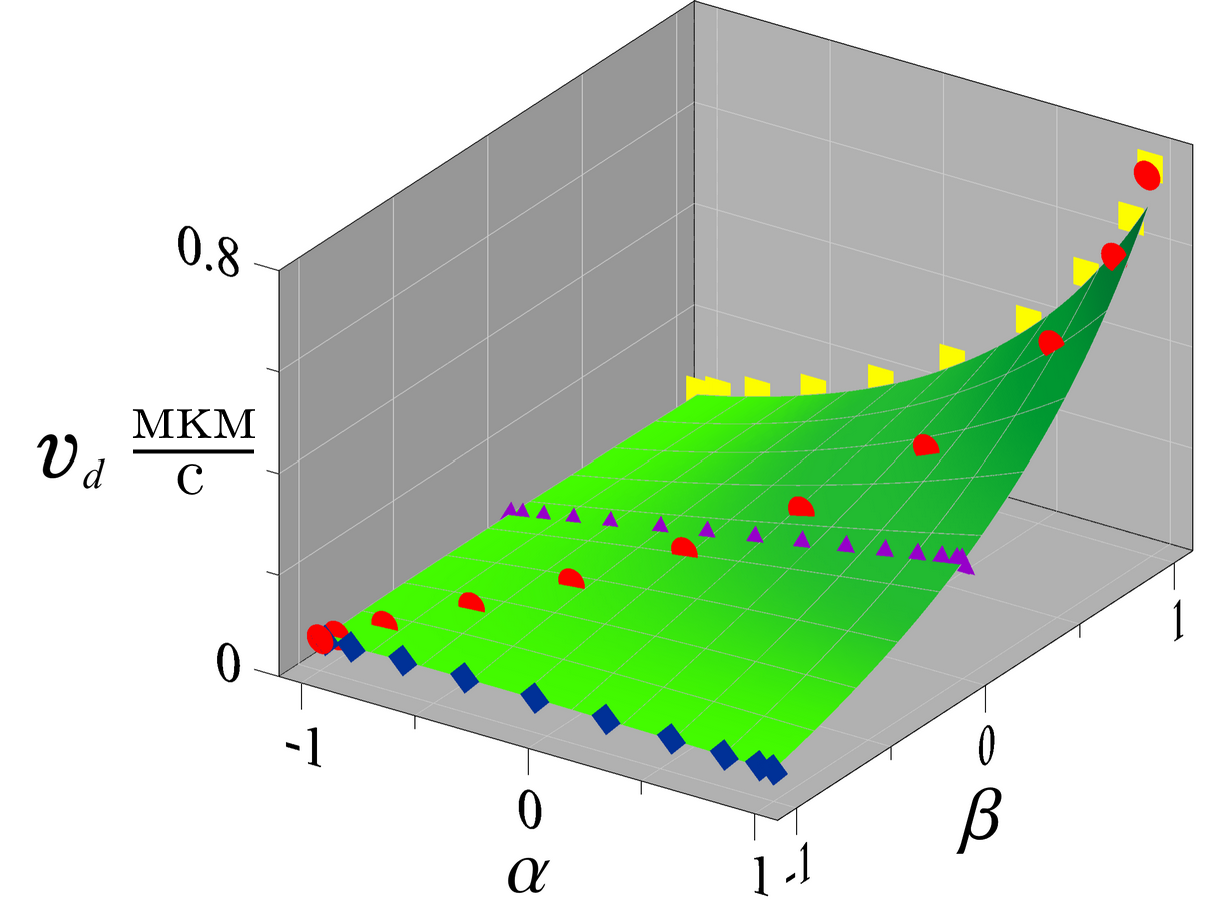
\includegraphics[width=1\linewidth]{genetic-noise/ru/fig2a} \\ а)
    \end{minipage}
    \hfill
    \begin{minipage}[b][][b]{0.49\linewidth}\centering
        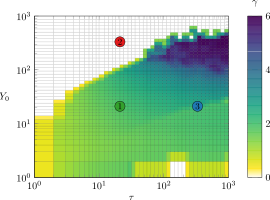
\includegraphics[width=1\linewidth]{genetic-noise/ru/fig2c} \\ б)
    \end{minipage}\\
    \begin{minipage}[b][][b]{0.49\linewidth}\centering
        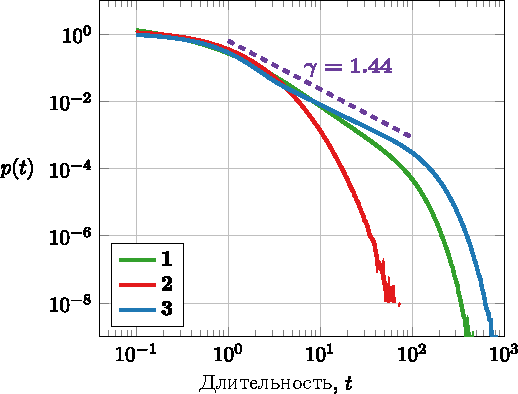
\includegraphics[width=1\linewidth]{genetic-noise/ru/fig2b} \\ в)
    \end{minipage}
    \hfill
    \begin{minipage}[b][][b]{0.49\linewidth}\centering
        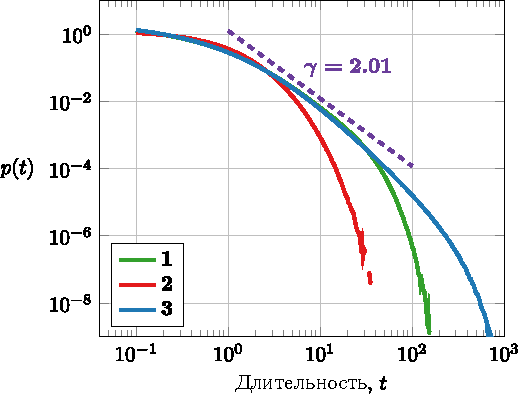
\includegraphics[width=1\linewidth]{genetic-noise/ru/fig2d} \\ г)
    \end{minipage}
    \caption{
        Показатель степени $\gamma$ для степенного участка плотности вероятности длительности CCW в зависимости от двух параметров: (a) среднего числа молекул CheY-P $Y_0$ и чувствительности $\alpha$ для фиксированного $\tau = 50$, (б) среднего числа молекул CheY-P $Y_0$ и времени корреляции $\tau$ при фиксированных $\alpha = 10$ и $K_0 = 1$. В белой области не наблюдается степенная асимптотика распределений длительности (гипотеза о наличии степенного участка отклоняется). Плотности для комбинаций параметров, отмеченных на панелях (а) и (б) цифрами 1,2,3, показаны на панелях (в) и (г) соответственно. 
    }\label{fig:pdf-gamma-grid-1}
\end{figure}

Далее рассмотрим более приемлемую с биологической точки зрения модель скорости перехода в соответствии с уравнением \cref{eq:turning-rates-kd}, которая имеет насыщение в интенсивностях переключения моторов. Для демонстрации крайних случаев эффекта насыщения рассмотрим ситуацию, когда уровень белка CheY-P находится на равновесном уровне $Y = Y_0$ и константа диссоциации меньше значения уровня равновесия $K_d < Y_0$. Результаты численного моделирования данной модели аналогично подтверждают, что медленная релаксация белка CheY-P вместе с более высокой чувствительностью интенсивности перехода от CCW к CW к изменению уровня белка приводят к появлению степенной асимптотики длительностей CCW, в то время как длительности CW остаются экспоненциально распределенными (Рис. \cref{fig:pdf-kd-powerlaw}).

\begin{figure}[ht]
    \centering
    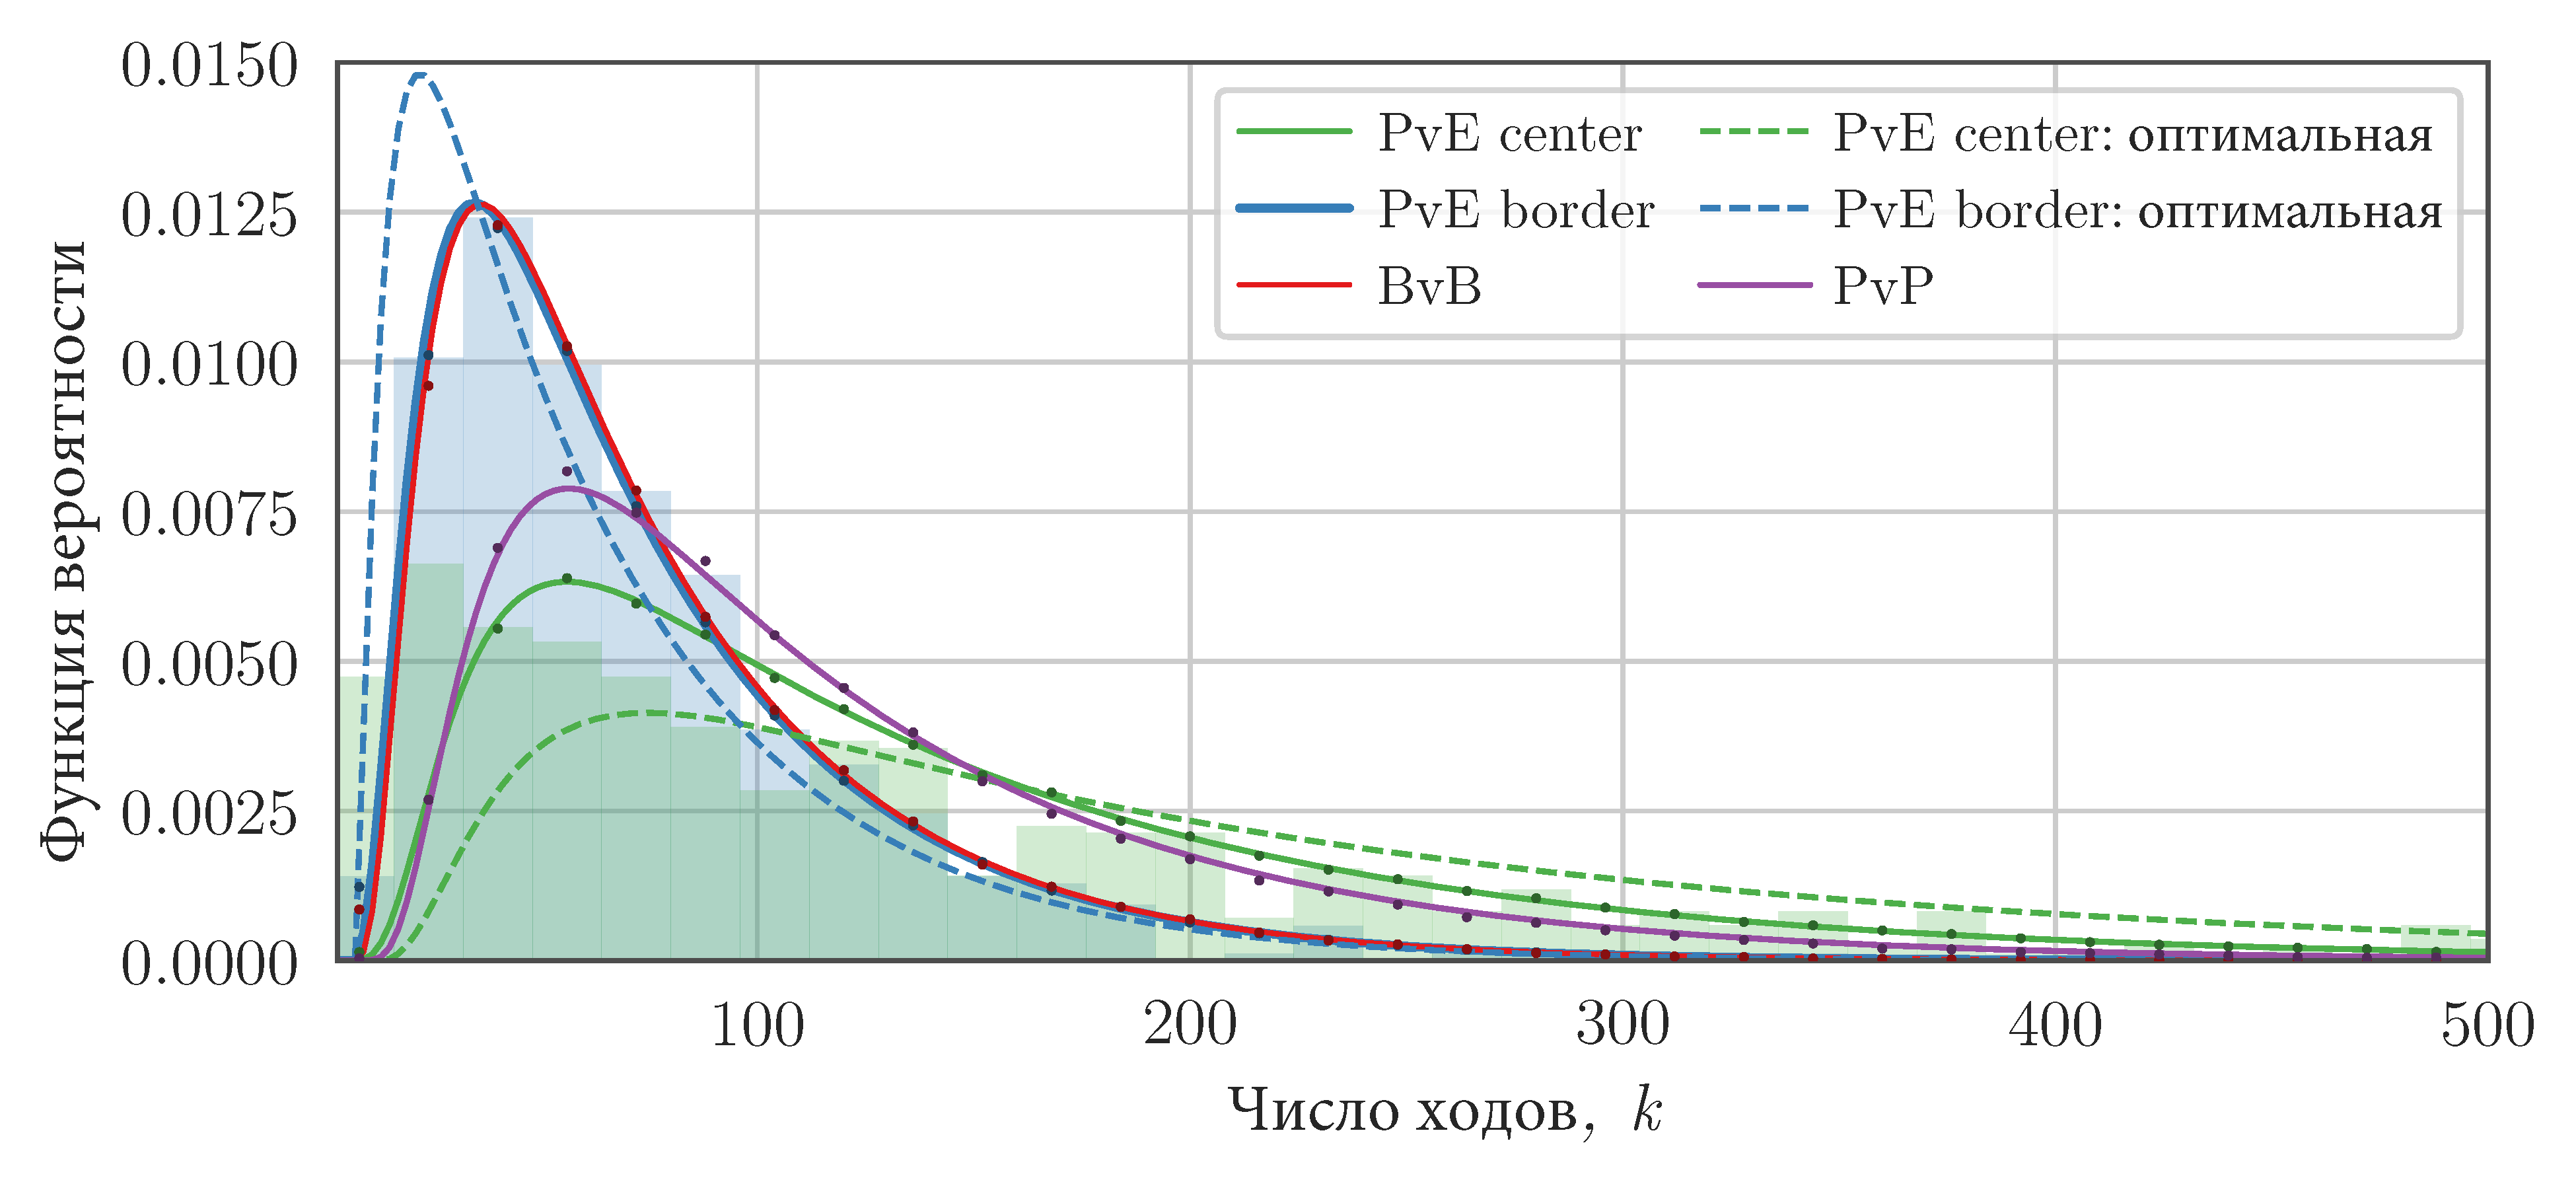
\includegraphics[width=0.5\linewidth]{genetic-noise/ru/fig3}
    \caption{
        Плотность вероятности длительности для состояний CW и CCW при $\alpha^- = 30$, $\alpha^+ = 1$, $Y_0 = 10$, $\tau = 50$, $K_d = 2$, $K^+_0 = 100$, $K^-_0 = 0.2$. Штриховая линия -- степенная зависимость с $\gamma = 3.18$, $R^2 = 0.999$, $N_{ccw} = 10^{11}$, $t \in [0.1, 20]$. На вставке повторно представлены плотности вероятностей длительностей с логарифмической шкалой по оси ординат.
    }
    \label{fig:pdf-kd-powerlaw}
\end{figure}



Систематическое исследование статистики в зависимости от значений параметров модели представлено на Рис. \cref{fig:pdf-gamma-grid-kd}. На плоскости параметров $(K_d, Y_0)$ выделяются две области, соответствующие двум различным вариантам поведения модели (Рис. \cref{fig:pdf-gamma-grid-kd}а). При $Y_0 < K_d$ эффект насыщения имеет слабое влияние, что приводит к сильному отклонению от степенной асимптотики по мере увеличения константы диссоциации. Степенная асимптотика проявляется при достаточно малых показателях $\gamma < 2$. Для $Y_0 > K_d$ введенный эффект насыщения приводит к большим значения показателя $\gamma > 4$ в степенной асимптотике. 

На другой плоскости параметров $(K_d, \alpha_-)$ степенная асимптотика сохраняется в широком диапазоне параметра чувствительности перехода от CCW к CW, $\alpha_-$ (Рис. \cref{fig:pdf-gamma-grid-kd}б). Аналогично выделяются режимы с относительно малыми $\gamma < 2$ и большими $\gamma > 4$ значениями показателя степени. Эти режимы обусловлены соотношением между средним числом молекул CheY-P, $Y_0$, и насыщением константы диссоциации $K_d$.

\begin{figure}[ht]
    \begin{minipage}[b][][b]{0.49\linewidth}\centering
        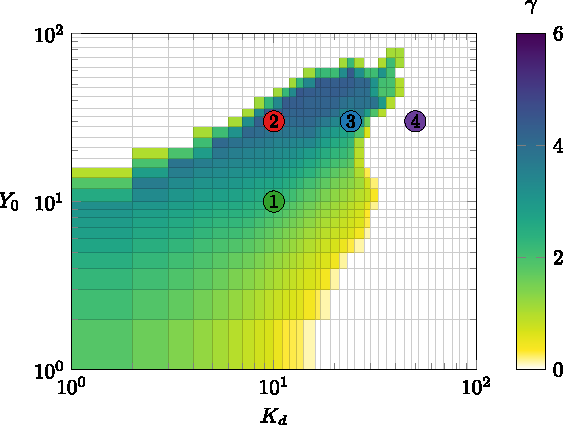
\includegraphics[width=1\linewidth]{genetic-noise/ru/fig4a} \\ а)
    \end{minipage}
    \hfill
    \begin{minipage}[b][][b]{0.49\linewidth}\centering
        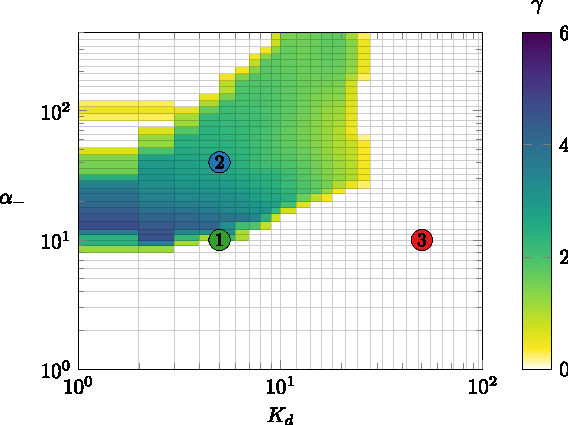
\includegraphics[width=1\linewidth]{genetic-noise/ru/fig4c} \\ б)
    \end{minipage}\\
    \begin{minipage}[b][][b]{0.49\linewidth}\centering
        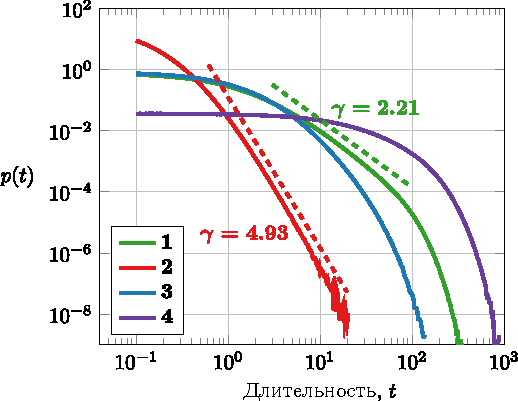
\includegraphics[width=1\linewidth]{genetic-noise/ru/fig4b} \\ в)
    \end{minipage}
    \hfill
    \begin{minipage}[b][][b]{0.49\linewidth}\centering
        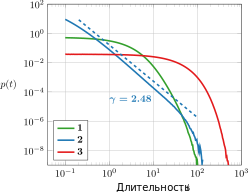
\includegraphics[width=1\linewidth]{genetic-noise/ru/fig4d} \\ г)
    \end{minipage}
    \caption{
        Показатель степени $\gamma$ для степенного участка плотности вероятности длительности CCW в зависимости от двух параметров: (a) константы насыщения $K_d$ и среднего числа молекул CheY-P $Y_0$ для фиксированного параметра $\alpha^- = 30$, (б) константы насыщения $K_d$ и параметра чувствительности $\alpha^-$ при фиксированном параметре $Y_0 = 10$. Остальные параметры модели были выбраны $\alpha^+=1$, $\tau=50$, $K^+_0=100$, $K^-_0=0.2$. В белой области не наблюдается степенная асимптотика распределений длительности (гипотеза о наличии степенного участка отклоняется). Плотности для комбинаций параметров, отмеченных на панелях (а) и (б) цифрами 1,2,3,4, показаны на панелях (в) и (г) соответственно. 
    }\label{fig:pdf-gamma-grid-kd}
\end{figure}


Таким образом биологически релевантная модель дает наиболее схожие с экспериментом показатели степени при коэффициенте диссоциации близком к константе диссоциации $K_d \approx Y_0$ при этом со значениями не превышающими $30$ молекул. Управление параметром $\alpha_-$ в свою очередь позволяет получить степенную асимптотику на большем числе декад, сохранив ее также на меньших промежутках длительностей нахождения в состоянии CCW.

Хотя применение подхода численного моделирования с применением алгоритма Гиллеспи обладает гибкостью к нахождению численных решений произвольных задач, временные затраты на вычисление ограничивают возможности применения модели. Подход full-counting statistics, впервые предложенный в работах по квантовой физике \cite{levitov_electron_1996}, позволяет независимо от природы основного кинетического уравнения оценить статистические свойства дискретной системы. Далее рассмотрим как данный подход может быть использован для вычисления статистики переключения моторов напрямую из интенсивностей перехода $K_x^\pm(Y)$ и $K_y^\pm(Y)$.

Рассмотрим кинетику модели, заданной уравнениями \cref{eq:chem,eq:turning}, в терминах марковских процессов с непрерывным временем \cite{tikhonov_markov_process_1977}. Диаграмма переходов представлены на рис. \cref{fig:transitions}. Состояние $Z(t)$ процесса в момент времени $t$ представляет собой двумерный вектор $Z = (X, Y)$, где первая компонента представляет направление вращения моторов $X = 0 \equiv \mathrm{CW}$ (по часовой стрелке) и $X = 1 \equiv \mathrm{CCW}$ (против часовой стрелки), а вторая компонента $Y$ -- количество молекул CheY-P. Тогда основное кинетическое уравнение для вектора вероятности $\mathrm{P}(Z, t) \equiv \mathrm{P}(X, Y, t)$ имеет вид:

\begin{equation}
    \begin{aligned}
        &\dot{\mathrm{P}}(\mathrm{CW},0,t)&=&-\left (\frac{Y_0}{\tau} + K_x^+(0) \right ) \mathrm{P}(\mathrm{CW},0,t) + K_x^-(0) \mathrm{P}(\mathrm{CCW},0,t)+&&\\
        &&&+\frac{1}{\tau}\mathrm{P}(\mathrm{CW},1,t),&&\\
        &\dot{\mathrm{P}}(\mathrm{CCW},0,t)&=&-\left (\frac{Y_0}{\tau} + K_x^-(0) \right ) \mathrm{P}(\mathrm{CCW},0,t) + K_x^+(0) \mathrm{P}(\mathrm{CW},0,t)&&\\
        &&&+\frac{1}{\tau}\mathrm{P}(\mathrm{CCW},1,t),&&\\
        &\dots&&\\
        &\dot{\mathrm{P}}(\mathrm{CW},Y,t)&=&-\left (\frac{Y_0+Y}{\tau} + K_x^+(Y) \right ) \mathrm{P}(\mathrm{CW},Y,t) + K_x^-(Y) \mathrm{P}(\mathrm{CCW},Y,t)+&&\\
        &&&+\frac{Y+1}{\tau}\mathrm{P}(\mathrm{CW},Y+1,t)+\frac{Y_0}{\tau}\mathrm{P}(\mathrm{CW},Y-1,t),&&\\
        &\dot{\mathrm{P}}(\mathrm{CCW},Y,t)&=&-\left (\frac{Y_0+Y}{\tau} + K_x^-(Y) \right ) \mathrm{P}(\mathrm{CCW},Y,t) + K_x^+(Y) \mathrm{P}(\mathrm{CW},Y,t)+&&\\
        &&&+\frac{Y+1}{\tau}\mathrm{P}(\mathrm{CCW},Y+1,t)+\frac{Y_0}{\tau}\mathrm{P}(\mathrm{CCW},Y-1,t),&&\\
    \end{aligned}
    \label{eq:master-transitions}
\end{equation}


\begin{figure}[ht]
    \centering
    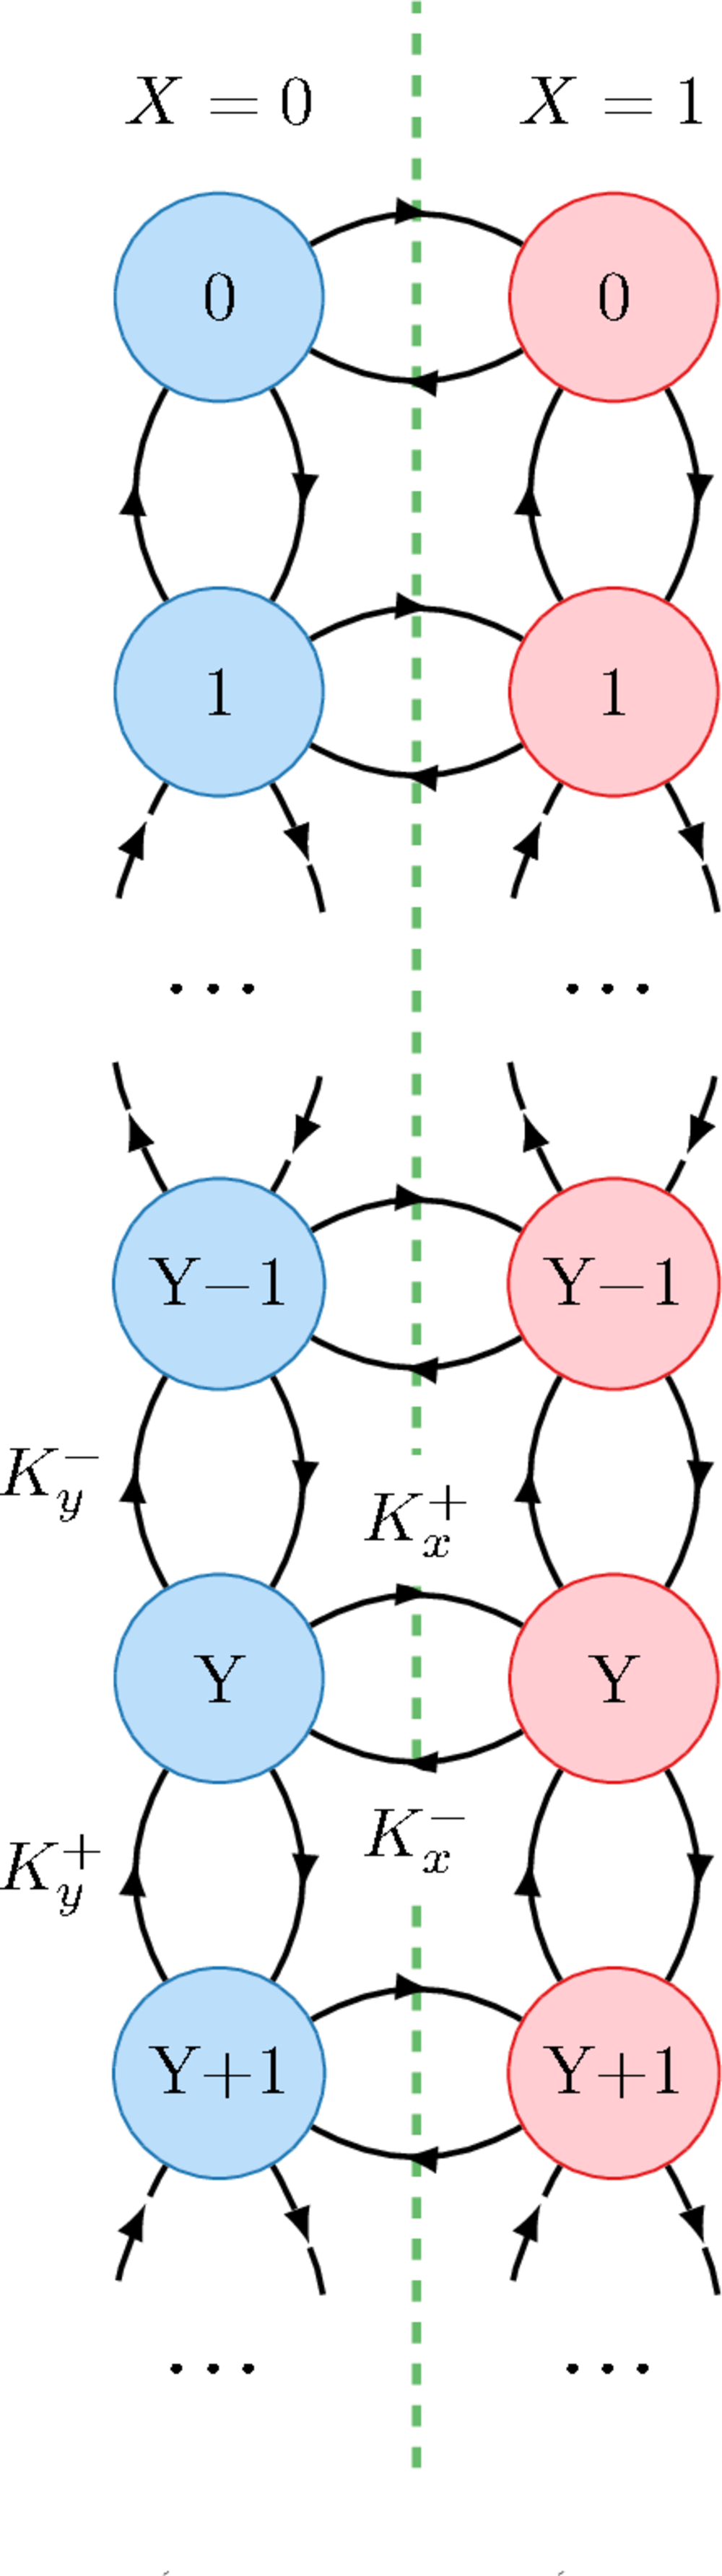
\includegraphics[width=0.25\linewidth]{genetic-noise/ru/fig0}
    \caption{
        Диаграмма переходов марковского процесса \cref{eq:master-transitions}, построенного для кинетической модели, описываемой уравнениями \cref{eq:chem,eq:turning}.
    }
    \label{fig:transitions}
\end{figure}

Примечательно, что наша модель служит обобщением жидкостной очереди, управляемой процессом рождения-смерти, предложенным ван Доорном, Ягерсом и де Витом \cite{van_doom_fluid_1988}. В терминах марковских процессов реакция \cref{eq:turning} представляет собой обмен вероятностью между двумя состояниями. Этот обмен можно рассматривать как обмен фиксированного количества несжимаемой жидкости между двумя баками со скоростями, определяемыми состоянием процесса рождения-смерти. В исходной постановке задачи был только один бак бесконечного объема и неограниченное количество жидкости. Длительность в состоянии CCW -- это время, которое одна молекула жидкости проводит в резервуаре <<1>>, прежде чем покинуть его. Введем вектор вероятности нахождения в каждом состоянии марковской цепи: 

\begin{equation}
    P(t) = \begin{bmatrix}
    P(X = \mathrm{CW}, Y = 0; t)\\
    P(X = \mathrm{CW}, Y = 1; t)\\
    P(X = \mathrm{CW}, Y = 2; t)\\
    ...\\
    P(X = \mathrm{CCW}, Y = 0; t)\\
    P(X = \mathrm{CCW}, Y = 1; t)\\
    P(X = \mathrm{CCW}, Y = 2; t)\\
    ...\\
    \end{bmatrix}
\label{eq:state-probs}
\end{equation}

Также для марковской цепи определим матрицу интенсивностей переходов $\boldsymbol{\mathrm{Q}}$ \cite{kapmen_stochastic_1990}. Тогда уравнение \cref{eq:master-transitions} представляется в компактной форме: 

\begin{equation}
    \boldsymbol{\mathrm{P}}(t) = \boldsymbol{\mathrm{Q}} \boldsymbol{\mathrm{P}}(t),
    \label{eq:master-transitions-compact}
\end{equation}

где матрица $\boldsymbol{\mathrm{Q}}$ состоит из суммы двух матриц: матрицы интенсивностей переходов процесса рождения-гибели для числа молекул, состоящей из двух одинаковых полубесконечных трехдиагональных блоков $\boldsymbol{\mathrm{Q}}_{BD}$; и матрицы, определяющей интенсивности переходов между сменой направления вращения моторов, состоящей из диагональных блоков:

\begin{equation}
    \boldsymbol{\mathrm{Q}}_{R} = 
    \begin{bmatrix} \mathrm{diag}\{-K^+_x (Y)\}&\mathrm{diag}\{+K^-_x (Y)\}\\ \mathrm{diag}\{+K^+_x (Y)\}&\mathrm{diag}\{-K^-_x (Y) \} \end{bmatrix}
    \label{eq:transition-block}
\end{equation}
где $\mathrm{diag}\{x_k\}$ -- обозначение полубесконечного диагонального матричного блока с элементами $x_k$ на диагонали.

Далее рассмотрим вероятность $P_A(t)$ отсутствия перехода из состояния CCW в состояние CW в течение времени $t$. Для этого определим вектор начального распределения по состояниям $(\mathrm{CCW}, Y)$:

\begin{equation}
    \boldsymbol{\mathrm{P_S}} = 
    \begin{bmatrix} P(\mathrm{CCW}, Y, 0)\\ \end{bmatrix}_Y
    \label{eq:start-prob}
\end{equation}

Для выбранного начального состояния, вероятность $P_A(t)$ может быть вычислена на основе вектора условных вероятностей обнаружения молекулы в момент времени $t$ в состоянии $(\mathrm{CCW}, Y)$ после $k$ переходов, рассмотренного при $k=0$ \cite{mordovina_full-counting_2013}: 
\begin{equation}
    \boldsymbol{\mathrm{P}}^{(k)}(t) = \begin{bmatrix} \boldsymbol{\mathrm{P}}^{(k)}(\mathrm{CCW}, Y, t)\end{bmatrix}_Y
    \label{eq:conditioned-transitions}
\end{equation}

Эволюция этого вектора при $k=0$ определяется соответствующим основным кинетическим уравнением:

\begin{equation}
    \dot{\boldsymbol{\mathrm{P}}}^{(0)}(t)=\boldsymbol{\mathrm{Q}}_{NT}\mathrm{P}^{(0)}(t) = \left (\boldsymbol{\mathrm{Q}}_{BD} - \boldsymbol{\mathrm{Q}}_{10} \right )
    \label{eq:conditioned-master-transtions}
\end{equation}
где $\boldsymbol{\mathrm{Q}}_{10} = \mathrm{diag}\{-K^-_x(Y)\}$ -- диагональная матрица с интенсивностями переходов из состояния CCW в состояние CW.

Тогда вероятность остаться в состоянии CCW выражается следующей суммой:
\begin{equation}
    P_A(t) = \sum_Y \mathrm{P}^{(0)}(\mathrm{CCW},Y,t)
    \label{eq:no-transition-prob}
\end{equation}

Матрица $\boldsymbol{\mathrm{Q}}_{NT}$ -- полубесконечная трехдиагональная матрица с положительными недиагональными элементами (матрица Якоби). Такая матрица имеет чисто вещественный невырожденный спектр ${\lambda_1, \lambda_2, ..., \lambda_i, ...}$. Наибольшее собственное значение отрицательное, $\lambda_1 < 0$, то есть существует <<утечка вероятности>> из состояния $X = \mathrm{CCW}$ в состояние $X = \mathrm{CW}$, так что основное кинетическое уравнение \cref{eq:master-transitions} не сохраняет норму вектора, и, соответственно, все остальные собственные числа также отрицательные $\lambda_i < 0$. 

Расчет вектора условной вероятности в любой момент времени может быть произведен путем спектрального разложения матрицы $\boldsymbol{\mathrm{Q}}_{NT}$:

\begin{equation}
    \boldsymbol{\mathrm{P}}^{(0)}(t) = \sum_i \alpha_i \exp(\lambda_i t) v_i,
    \label{eq:solution-no-transition-prob}
\end{equation}
где $\alpha_i=w_i^T \boldsymbol{\mathrm{P_S}}$, $\boldsymbol{w_i}$ -- набор левых собственных векторов матрицы $\boldsymbol{\mathrm{Q}}_{NT}$, $\boldsymbol{v_i}$ -- набор правых собственных векторов матрицы $\boldsymbol{\mathrm{Q}}_{NT}$. Затухание $P_A(t)$ с увеличением времени происходит монотонно из-за свойств спектра.

Для вычисления плотности вероятности $p(t)$ длительности нахождения в состоянии CCW, необходимо вычислить $P_A(t)$ для начального вектора $\boldsymbol{\mathrm{P_S}}$, соответствующего распределению по состояниям $Y$ в момент, когда происходит переход из состояния CW в состояние CCW.
Тогда плотность вероятности записывается следующим образом:

\begin{equation}
    p(t) = -\dot{P_A}(t) = \sum_Y \sum_i -lambda_i \alpha_i \exp(\lambda_i t) (\boldsymbol{v_i})_Y,
    \label{eq:solution-no-transition-pdf}
\end{equation}

Для получения начального распределения, в момент перехода из состояния CW в состояние CCW, необходимо найти стационарное распределения $\boldsymbol{\mathrm{P_{st}}}$ полной марковской цепи:

\begin{equation}
    \boldsymbol{\mathrm{Q}} \boldsymbol{\mathrm{P_{st}}} = \boldsymbol{0},
    \label{eq:transitions-stationary}
\end{equation}
где $\boldsymbol{0}$ -- нулевой полубесконечный вектор.

Подвектор, соответствующий состоянию CW: ${P_{st}(CW, Y)}$, будет определять вероятность нахождения системы в состоянии $Y$ при условии ее нахождения в CW. Вероятность перехода системы из $(\mathrm{CW}, Y)$ в $(\mathrm{CCW}, Y)$ пропорциональна интенсивности перехода $K_x^+(Y)$. Однако для системы из бесконечного числа состояний относительная частота перехода в общем случае не определена. В связи с этим осуществим переход к конечному числу состояний, в которых сконцентрирована вероятность нахождения системы. 

\begin{equation}
    P_x^+(Y)=\frac{K_x^+(Y)}{\sum_{Y\in W} K_x^+(Y)},
    \label{eq:cw-to-ccw-prob}
\end{equation}
где $W$ -- конечный набор состояний числа молекул $Y$, в которых сконцентрирована вероятность нахождения системы. Оценка на погрешность вычисленных вероятностей в зависимости от подмножества выбранных состояний при переходе к конечномерной системе дается в теореме о проекции марковской цепи на конечное число состояний \cite{munsky_finite_2006}. Также в работе предлагается алгоритм, который дает возможность определить достаточное число состояний для получения необходимой точности.

Тогда по теореме Байеса вероятность нахождения системы в состоянии $(\mathrm{CCW}, Y)$ при условии, что до этого она была в $(\mathrm{CW}, Y)$:
\begin{equation}
    P_S(Y)=\frac{P_{st}(\mathrm{CW}, Y) P_x^+(Y)}{\sum_{Y\in W} P_{st}(\mathrm{CW}, Y) P_x^+(Y)},
    \label{eq:start-prob-solution}
\end{equation}

Далее было проведено сравнение результатов расчета плотностей вероятностей длительностей методом Гиллеспи и расчета прямым методом, полученным из теории Марковских цепей и подхода full-counting statistics. Вычисление прямым методом сводится к нахождению собственных чисел и векторов матрицы $\boldsymbol{\mathrm{Q}}_{NT}$ и нахождению стационарного распределения марковской цепи. На рисунке \cref{fig:gillespi-vs-direct}. Рассчитанное таким образом распределение длительностей полностью совпадает с распределением, полученным при расчете статистики по множеству реализаций стохастическим алгоритмом Гиллеспи.

\begin{figure}[ht]
    \centering
    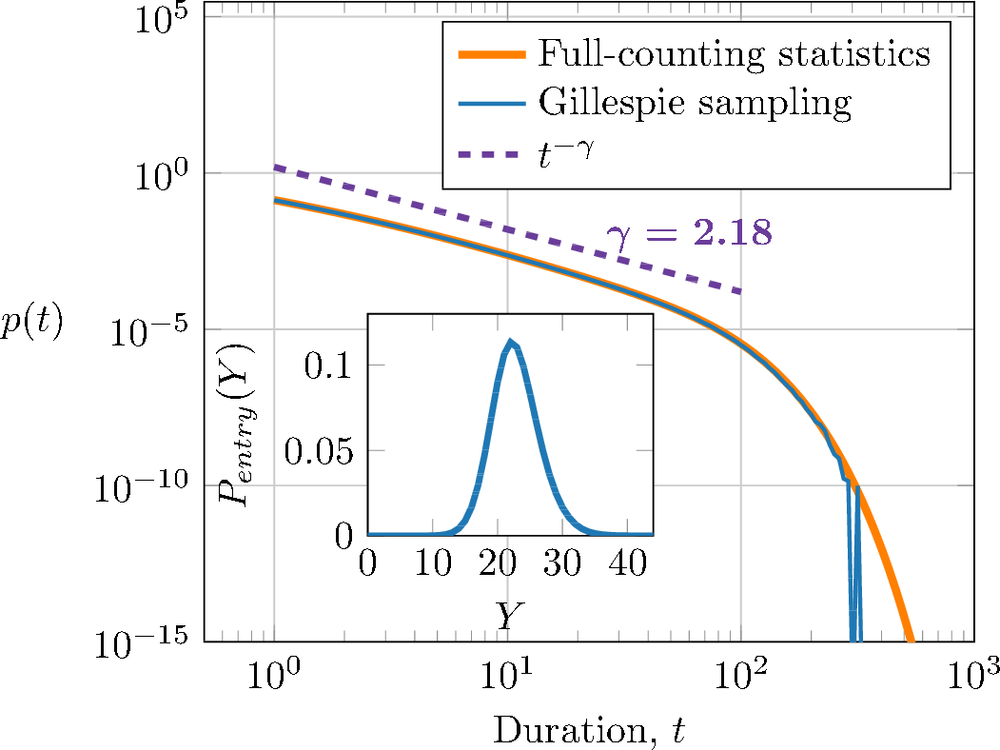
\includegraphics[width=\linewidth]{genetic-noise/ru/fig1c.png}
    \caption{
        Плотности вероятности длительностей CCW, полученные с применением двух подходов: оранжевая линия -- подход full-counting statistics для процесса, описываемого основным уравнением \cref{eq:conditioned-master-transtions}, с усечением при $Y_{max} = 100$; синяя линия -- метод Гиллеспи для исходной кинетической модели \cref{eq:chem,eq:turning}. На вставке показано распределение вероятности $P_S(Y)$ для начального распределения состояний CCW относительно числа молекул $Y$, \cref{eq:start-prob-solution}. Параметры модели были выбраны эквивалентно параметрам на рисунке \cref{fig:duration-pdf}б.
    }
    \label{fig:gillespi-vs-direct}
\end{figure}

\section{Модель движения бактерии с двумя чередующимися событиями поворота}\label{sec:ch2/sec2}

Рассмотренная в предыдущем разделе бактерия E.~coli обладает паттерном движения, состоящим из двух стадий: прямолинейного движения и вращения на одном месте. Однако в зависимости от среды обитания и других факторов эволюционно бактерии выработали различные паттерны движения для ориентации в пространстве. Примером бактерии с характерно другим паттерном служит вид V.~alginolyticus, обитающий в морской среде. Паттерн движения V.~alginolyticus состоит из трех этапов: прямолинейное движение, реверсивное движение и быстрый разворот \cite{xie_bacterial_2011}. В этом паттерне бактерия движется некоторое время вперед, затем направление вращения моторов жгутиков меняются на противоположное и бактерия осуществляет реверсивное движение. При реверсивном движении жгутики бактерии имеют механическую нестабильность, что приводит к третьему этапу разворота бактерии \cite{taute_high-throughput_2015}. Пример движения бактерии реконструированного в эксперименте, приведен на рисунке \cref{fig:vibrio-trajectories}.

Дополнительно было показано, что средний угол разворота зависит от размера клетки, при этом более крупные клетки имеют большие углы разворота \cite{taute_high-throughput_2015}. Это означает, что более крупные клетки стабилизируют движение за счет противодействия силе вязкого сопротивления, действующей на тело клетки, и соответственно угол их поворота получается ближе к реверсивному. 


Применяя формализм де Жена \cite{de_gennes_chemotaxis_2004}, построим модель, описывающую движение бактерии с двумя чередующимися событиями поворота.

Пусть паттерн движения состоит из 4 этапов: 
\begin{enumerate}
  \item "Вперед-1": прямолинейное движение в некотором направлении.
  \item "$\alpha$-поворот": поворот на некоторый случайный угол $\Delta\phi_1$ при котором средний косинус угла равен $\alpha$, то есть $M[\cos (\Delta\phi_1)]=\alpha$.
  \item "Вперед-2": прямолинейное движение в новом направлении.
  \item "$\beta$-поворот": поворот на некоторый случайный угол $\Delta\phi_2$ при котором средний косинус угла равен $\beta$, то есть $M[\cos (\Delta\phi_2)]=\beta$.
\end{enumerate}

Скорость движения бактерии при прямолинейном движении рассматривается как константа, одинаковая для 1 и 3 этапов. Однако, существуют другие виды бактерий, например, P.~putida, обладающие различной скоростью движения чередующихся прямолинейных движений \cite{theves_bacterial_2013}. В данной модели скорости выбраны одинаковыми, чтобы сконцентрироваться на влиянии именно паттерна движения, состоящего из двух различных углов.

Рассматриваемый $\alpha-\beta$ паттерн движения экспериментально наблюдается у различных видов бактерий, таких как P.~haloplanktis, V.~coralliilyticus \cite{son_bacteria_2013}, C.~crescentus \cite{liu_helical_2014}, S.~putrefaciens \cite{stocker_reverse_2011} и других. 

В данном разделе детали модели будем основывать на экспериментальных наблюдениях за бактериями V.~alginoulticus. Экспериментально было продемонстрировано \cite{altindal_implications_2011}, что в отсутствии химического градиента данный вид бактерий демонстрирует среднее время участка прямолинейного движения, одинаковое для первого и третьего этапа паттерна, равное $\tau \approx 0.3s$. Наблюдаемое в эксперименте распределение длительностей представляет собой экспоненциальное распределение, однако в области коротких времен распределение часто отклоняется от экспоненциального. В рассматриваемой модели будем использовать упрощенное предположение о том, что распределение следует экспоненциальному закону с показателем $\lambda_0=\frac{1}{\tau_{run}}$. Такой выбор связан с упрощением предложенного аналитического анализа. Длительности же второго и четвертого этапов, характеризующих процесс вращения бактерии на одном месте, на порядок меньше, чем длительности прямолинейного движения, в связи с чем ими обычно пренебрегают в моделях \cite{block_adaptation_1983}. В предложенной модели будем рассматривать повороты как мгновенные события.

Движение бактерии сопряжено с тепловым шумом жидкости и активными процессами в моторах бактерии, что вызывает отклонения от строго прямолинейного движения. Экспериментально было показано, что такие отклонения согласуются с броуновской вращательной диффузией \cite{berg_chemotaxis_1972}, которая описывается константой $D_r$. Значение константы может быть экспериментально измерено и ее значение согласуется со значением для броуновской вращательной диффузии пассивной частицы с размером характерным для бактерии. Влияние ротационной диффузии может отклонять за этап прямолинейного движения направляющий вектор до $30^\circ$. 

В отсутствии химических веществ траектория для такого паттерна движения представляет собой случайное блуждание, характеризующееся корреляционной функцией скорости и эффективной постоянной долговременной диффузии бактерии, аналитические выражения для которых были найдены в работе Йоханнес Тактикос \cite{taktikos_how_2013}. 

В случае наличия химических веществ в среде, бактерия способна направлять свое случайное блуждание в направлении химического аттрактанта за счет хемосенсорной системы. Работа этой системы обеспечивает интеграцию сигнала во времени и ответную реакцию с некоторой задержкой, изменяющую направление вращения моторов жгутиков. При движении бактерии в направлении градиента длительность этапа прямолинейного движения увеличивается, позволяя бактерии продолжать движение в благоприятную сторону. 

Основной линейной моделью хемотаксиса бактерии является модель де Жена \cite{de_gennes_chemotaxis_2004}, которая связывает частоту переключения направления вращения моторов $\lambda(t)$ со значением концентрации химического вещества $c(t)$, измеренного сенсорами бактерии:

\begin{equation}
    \begin{aligned}
        \lambda(t)=\lambda_0 \left ( 1 - \int_{-\infty}^t R(t-\tau)c(\tau)d\tau \right ),
    \label{eq:turning-frequency}
    \end{aligned}
\end{equation}
где $\lambda_0=\frac{1}{\tau_{run}}$ -- частота переключения в отсутствии химических веществ, $R(t)$ -- внутренняя функция отклика бактерии. В случае с видом бактерий E.~coli функция отклика бактерии была измерена экспериментально в работе \cite{block_adaptation_1983} и аналитически представима в следующем виде:

\begin{equation}
    \begin{aligned}
        R(t) = W \lambda_0 e^{-\lambda_0t} \left ( 1 - \frac{lambda_0T}{2} - \left (\frac{lambda_0T}{2}\right )^2 \right )
    \label{eq:response-ecoli}
    \end{aligned}
\end{equation}
где $W$ характеризует силу отклика бактерии.  

Важное свойство функции отклика состоит в способности бактерии подстраиваться под фоновую концентрацию химического вещества и относительно нее распознавать малый градиент. Для учета отсутствия влияния однородной концентрации на частоту функция отклика должны обладать следующим свойством:  
\begin{equation}
    \begin{aligned}
        \int_{-\infty}^{\infty} R(\tau)d\tau = 0
    \label{eq:response-ecoli-zero}
    \end{aligned}
\end{equation}
Тогда в уравнении \cref{eq:turning-frequency} при постоянной концентрации $c(t)\equiv const = C$ интеграл также обращается в ноль и $\lambda(t)=\lambda_0$. Таким образом, если функция отклика обладает указанным свойством, то малые изменения $\Delta c(t)$ относительно фоновой концентрации $C$ в измеряемой концентрации вещества $c(t)=C+\Delta c(t)$ влияют на частоту переключений $\lambda(t)$ независимо от величины $C$. 

Ранее 


\section{Скорость смещения бактерий}\label{sec:ch2/sec3}
\section{Численная симуляция движения ансамбля бактерий}\label{sec:ch2/sec4}

